% An infinite prime σ : K → ℂ lifting to an infinite prime τ : L → ℂ
% in an extension L/K, as a commuting triangle.
% Source: book/tex/alg-NT/artin.tex (§ Infinite primes in
% extensions) — tikzcd.
\documentclass[border=2mm]{standalone}
\usepackage{tikz}
\usetikzlibrary{arrows.meta}
\usepackage{amssymb}
\usepackage{amsmath}
\begin{document}
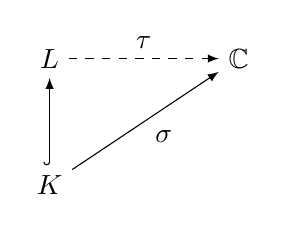
\begin{tikzpicture}[>=latex]
  \node (L) at (0,1.6) {$L$};
  \node (C) at (2.4,1.6) {$\mathbb{C}$};
  \node (K) at (0,0) {$K$};
  \draw[->, dashed] (L) -- (C) node[midway,above] {$\tau$};
  \draw[{Hooks[right]}->] (K) -- (L);
  \draw[->] (K) -- (C) node[midway,below right] {$\sigma$};
\end{tikzpicture}
\end{document}
